%%%%%%%%%%%%%%%%%%%%%%%%%%%%%%%%%%%%%%%%%%%%%%%%%%%%%
%% LaTeX2e Template by Stephen Iota (iota@usc.edu) %%
%%%%%%%%%%%%%%%%%%%%%%%%%%%%%%%%%%%%%%%%%%%%%%%%%%%%%
\documentclass{article}
\usepackage{geometry}
\usepackage[utf8]{inputenc}
%%%%%%%%%%%%%%%%%%%%%%%%%%%%%%%%%%%%%%%%%%%%%%%%%%%%%
%% LaTeX2e Template by Stephen Iota (iota@usc.edu) %%
%%%%%%%%%%%%%%%%%%%%%%%%%%%%%%%%%%%%%%%%%%%%%%%%%%%%%
\usepackage[utf8]{inputenc}
\usepackage{amsmath, amssymb, amsthm}
\usepackage{physics}
%\usepackage{algorithm}
%\usepackage[noend]{algorithmic}
\usepackage{mathtools}  % for boxed answers in align environments
%\usepackage{cancel}
\usepackage{graphicx}
\usepackage[shortlabels]{enumitem}  % change labels in enum/item envs, [noitem[list]sep]
%\usepackage[labelfont=bf,font=small]{caption}
\usepackage[dvipsnames]{xcolor}
%\usepackage[big]{titlesec}  % [small,medium,big]
%\usepackage{fancyhdr}
%\usepackage[noadjust]{cite}
%\usepackage{tikz}
\usepackage[colorlinks=true,
            citecolor=NavyBlue!90!black,
            linkcolor=green!50!black,
            urlcolor=green!50!black,
            hypertexnames=false]{hyperref}

%%%%%%%%%%%%%%%%%%%%%%%
%%%% MISC COMMANDS %%%%
%%%%%%%%%%%%%%%%%%%%%%%
\graphicspath{{./figures/}} % Setting the graphics path
\newcommand{\email}[1]{\texttt{\href{mailto:#1}{#1}}}
\newcommand{\pref}[1]{[\ref{#1}]}

%%%%%%%%%%%%%%%%%%%%
%%% FRONT MATTER %%%
%%%%%%%%%%%%%%%%%%%%
\def\makemytitle{
	\begin{center}
        {\LARGE \textsc{\nclass}: \npset}%\textbf{\npset}}
    \end{center}
    \bigbreak
    \begin{center}
        \nauthor        \\
        \email{\nemail} \\
		\nthanks        \\
        \ndate
    \end{center}
}

%%%%%%%%%%%%%%%%%%%%%%%%%%%%%%%%
%% My commands & environments %%
%%%%%%%%%%%%%%%%%%%%%%%%%%%%%%%%
%\numberwithin{equation}{section}
\theoremstyle{plain}
\newtheorem{problem}{Problem}
%\numberwithin{problem}{Problem}
\theoremstyle{definition}
%\swapnumbers % `2.1 Solution' instead of `Solution 2.1'
\newtheorem*{solution}{Solution}
%\numberwithin{solution}{solution}
\newtheorem{question}{Problem}
\renewcommand\qedsymbol{$\blacksquare$}

%%%%%%%%%%
%% MISC %%
%%%%%%%%%%
\newcommand{\nextproblem}[0]{\bigbreak}


%%%%%%%%%%%%%%%%%%%%%%%
%%%% MATH COMMANDS %%%%
%%%%%%%%%%%%%%%%%%%%%%%
\newcommand{\transpose}[1]{\ensuremath{#1^T}}
\newcommand{\colvec}[1]{\ensuremath{\begin{pmatrix} #1 \end{pmatrix}}}
\newcommand{\eye}[0]{\ensuremath{\mathbb{I}}}
\newcommand{\R}[0]{\ensuremath{\mathbb{R}}}
\newcommand{\union}[0]{\cup}
\newcommand{\intersect}[0]{\cap}
\newcommand{\set}[1]{\ensuremath{\{#1\}}}
\newcommand{\compl}[1]{\ensuremath{#1^{c}}}
\newcommand{\factorial}[1]{\ensuremath{#1!}}

\DeclareMathOperator{\Cov}{Cov}


\usepackage{caption}
\usepackage{subcaption}

%%%%%%%%%%%%%
%%% Begin %%%
%%%%%%%%%%%%%
\begin{document}

    \begin{center}
        {\LARGE \textsc{cs545 Robotics HW4:} \textbf{Path planning with RRTs}}
    \end{center}

    \bigbreak

    \begin{center}
        Stephen Iota%\footnote{SID: \texttt{6862013543}}
        \\
        \email{iota@usc.edu}
        \\
        \texttt{SID:} \texttt{6862013543}
        \\
        \today
    \end{center}

    \bigbreak

    \section*{Planar RRT}
    See figure~\ref{fig:planar_rrt}.

    \begin{figure}[p]
        \centering
        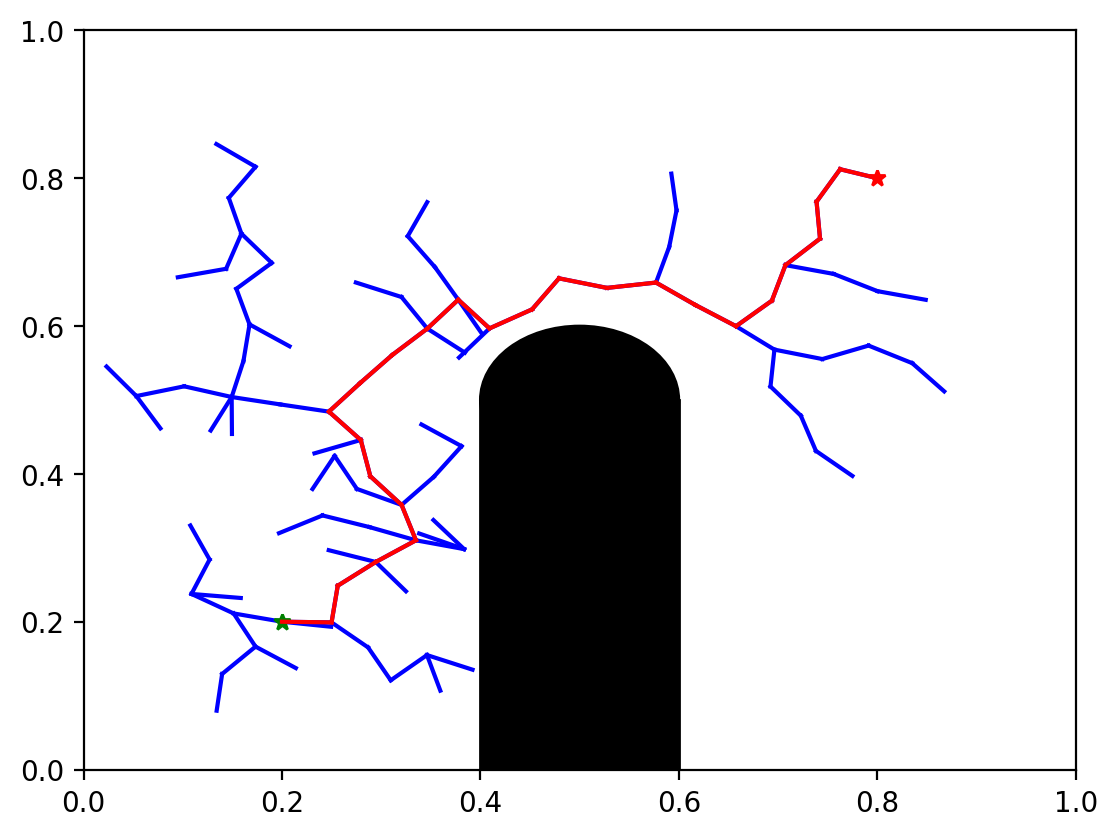
\includegraphics[width=0.8\linewidth]{planar_rrt.png}
        \caption{Visualization of the RRT search algorithm in 2D (with default config.).}
        \label{fig:planar_rrt}
    \end{figure}

    \section*{Questions}

    \begin{enumerate}
        \item[(1)] \textit{Why is the path returned by the RRT not guaranteed to be optimal?} \\
                    The RRT algorithm makes no claims about optimality. The algorithm returns the first path it finds that connects the starting point to the goal point. It does this not in a systematic way, but by sampling randomly.  There will likely exit a shorter, more efficient path to the goal state.
        \item[(2)] \textit{What effect will increasing $\delta$ have on the performance of the RRT?} \\
                    If stepsize $\delta$ is greater than the width of the obstacle, the algorithm may try to step over the obstacle, which would in reality cause the agent to crash.  However if you can ensure there are no obstacles, the algorithm will converge to a path quicker with a larger $\delta$. 
        \item[(3)] \textit{What effect will increasing the bounds of the search space have on the performance
        of the RRT? How about increasing the number of dimensions of the search space?} \\
                    Increasing either of these factors will decrease the performance of RRT; the algorithm will be subject to the curse of dimensionality. In higher dimensions or with a larger sample space, it is much less likely the algorithm will sample a valid path, especially if the goal posiiton is far away from the initial posiiton.
        \item[(4)] \textit{Why is it important to have a relatively small $\delta$?} \\
                    A relatively small $\delta$ ensures the algorithm will not attempt to cross over any obstacles, causing the agent to collide.
    \end{enumerate}

\end{document}